%  This is a example presentation using the provided beamertheme
%  <jacknjo> compiled with pdflatex.
%
%  Copyright (C) 2016  Florian Hofmann - JacknJo
%
%  This file is part of the beamertemplate jacknjo which 
%  can be found at <https://github.com/JacknJo/jacksbeamertheme>.
%
%  The theme and this example is free software: you can
%  redistribute it and/or modify it under the terms of the GNU 
%  General Public License as published by the Free Software 
%  Foundation, either version 2 of the License, or (at your 
%  option) any later version.
%
%  The theme is distributed in the hope that it will be useful,
%  but WITHOUT ANY WARRANTY; without even the implied warranty of
%  MERCHANTABILITY or FITNESS FOR A PARTICULAR PURPOSE.  See the
%  GNU General Public License for more details.
%
%  You should have received a copy of the GNU General Public 
%  License along with this theme. 
%  If not, see <http://www.gnu.org/licenses/>.

\documentclass[
	12pt, 				% fontsize; available are 10pt, 11pt, 12pt
	t,					% define to start from top of the page
	aspectratio=169,	% page aspectratio; available are 43, 169, 54, 32, 1610, 149
	%handout			% define if you only want a handout version without the overlay makros
	]{beamer}
	
% ##### choose theme and define it's color #####
\usetheme{jacknjo}
\colortheme{3} % [0] blue; [1] orange; [2] green; [3] red; [4] turquoise;

% ##### language and encoding #####
\usepackage[T1]{fontenc}
\usepackage[ngerman]{babel} % by using the babel package, date shows as dd Month yyyy

% ##### other packages you might need #####
\usepackage{lipsum}
%\usepackage{minted}		% Can be used for source code highlighting. Mention the workaround in file <var/mintedExample.tex>

\usepackage{datetime}
\ddmmyyyydate \renewcommand{\dateseparator}{.}


% The fastcompile command only matters if you want to change the font. If you don't want to just leave it as 0. Then you will have to compile your project with the lualatex compiler and fastcompile must be set to 1. Also one of the following \setmainfont{fontname} lines has to be uncommented (notice that the .ttf or .otf font has to be installed on your system)
\newcommand{\fastcompile}{0} % [0] pdflatex; [1] lualatex
\ifnum\fastcompile=0
	\usepackage[utf8]{inputenc}
\else
	\usepackage{fontspec}
	%X##### simple font, straight letters, mathmode - ok
	%\setmainfont[Mapping=tex-text]{Lucida Sans} 
	
	%X##### similar to ubuntu, less bold mathmode - ok
	%\setmainfont[Mapping=tex-text]{Trebuchet MS}
	
	%X##### bold text, not for math mode
	%\setmainfont[Mapping=tex-text]{Ubuntu}  % Ubuntu Light as alternative
	
	%X#####
	%\setmainfont[Mapping=tex-text]{Liberation Sans}
	
	%X##### great looking, favorite
	%\setmainfont[Mapping=tex-text]{Open Sans} 
	
	%X##### good looking, strict and standard font
	%\setmainfont[Mapping=tex-text]{Fira Sans} 
	
	%X##### great looking, playful round & easy to read, no bold font!
	%\setmainfont[Mapping=tex-text]{ABeeZee}\renewcommand{\textbf}[1]{\textit{#1}}
	
	%X##### playful font, not so serious
	%\setmainfont[Mapping=tex-text]{Josefin Sans SemiBold} 
	
	\let\sfdefault\rmdefault
\fi


% ##### custom environments #####
\newenvironment{blocksatz}{\begin{justify}\vspace*{-0.475cm}}{\end{justify}}

% ##### custom commands #####
\newcommand{\pictureat}[4]{%
	\only<+(1)->{
		\begin{textblock*}{\paperwidth}(#1, #2)%
			\includegraphics[#3]{#4}%
		\end{textblock*}}}
		
% This custom command can be used with the theme and provides a zoom in of the specified picture
% it has to be specified manually by the first command if width = \pagewidth or height = \pageheight
% to fit on the screen. The second command specifies the path to the picture.
\newcommand{\fillpic}[2]{
	\clearpage
	\begin{textblock*}{\paperwidth}(0pt,0pt)
		\begin{tikzpicture}
		\useasboundingbox (0, 0) rectangle(\paperwidth,\paperheight);
		\fill [color = black, fill opacity=0.75](0, 0) rectangle(\paperwidth,\paperheight);
		\node (label) at (0.5\paperwidth,0.5\paperheight){\includegraphics[#1]{#2}};
		\end{tikzpicture}
	\end{textblock*}
}

\newcommand{\myCheck}{
	\begin{tikzpicture}[y=0.80pt, x=0.80pt, yscale=-0.2, xscale=0.2, inner sep=0pt, outer sep=0pt]
	\path[draw=myCol2,line join=round,line cap=round,miter limit=4.00,line
	width=2.100pt,rounded corners=0.0000cm] (295.0000,420.9336) rectangle
	(395.0000,520.9336);
	\path[draw=myCol1,line join=miter,line cap=round,miter limit=4.00,even odd
	rule,line width=2.5pt] (307.9327,463.8016) -- (341.2462,507.1091) --
	(410.6824,425.8807);
	\end{tikzpicture}}

\newcommand{\myUnCheck}{
	\begin{tikzpicture}[y=0.80pt, x=0.80pt, yscale=-0.2, xscale=0.2, inner sep=0pt, outer sep=0pt]
	\path[draw=myCol2,line join=round,line cap=round,miter limit=4.00,line
	width=2.100pt,rounded corners=0.0000cm] (295.0000,420.9336) rectangle
	(395.0000,520.9336);
	\end{tikzpicture}}

% ##### Titlepage settings - positive and negative lengths are accepted #####
\setlength{\titleoffset}{0cm}
\setlength{\subtitleoffset}{0pt}
\setlength{\dateoffset}{0cm}

% ##### Frame settings - positive and negative lengths are accepted #####
\setlength{\framesubtitleoffset}{0pt}
\setlength{\frametitleoffset}{0.05cm}
\setlength{\frametextoffset}{0.1cm}
\setlength{\framefootlineoffset}{0cm}

% ##### Title page Information ##### 
\title{The Fleye \\Groundstationsoftware}
\subtitle{Änderungen und Neuerungen}
\author{%
		Florian Hofmann
		}
\date{Friedrichshafen\\\today}

\newcommand{\middleText}{\copyright Florian Hofmann - GPL2.0}

% ##### Use this line to place your logo. {posx}{posy}{options}{filename}
\renewcommand{\uselogo}{1} %uncommented -> logo on ; commented -> logo off
    \setlength{\logox}{\paperwidth  - 1.25cm}
    \setlength{\logoy}{\paperheight - 0.62cm}
    \newcommand{\logographics}{
\includegraphics[width=1.75cm]{figures/fleyeLogo2.png}}
    
% ##### Add your literature.bib here #####
\addbibresource{var/literature.bib}


\begin{document}
		
	\begin{frame}[noframenumbering]
		\titlepage
	\end{frame}


	\begin{frame}{Gliederung}
		\tableofcontents
	\end{frame}


%\outlinesection{Gliederung}

	% To use minted in a beamer theme you have to use the following workaround and compile with the -shell-escape flag!
	%	\definecolor{bg}{rgb}{0.95,0.95,0.95}
	\newminted{python}{fontsize=\scriptsize, 
		linenos,
		numbersep=8pt,
		gobble=4,
		frame=lines,
		bgcolor=bg,
		framesep=3mm} 

	% check here: http://nochair.net/posts/2011/05-05-fragile-latex-beamer.html
	\defverbatim[colored]\exampleCode{
		\begin{pythoncode}
			import numpy as np
			import pylab as pl
			
			def f_x(x):
			return np.exp(x)+x**2-5*x
			
			def approx_f(x):
			return 1 -4*x +3./2*x**2
			
			xvals = np.arange(-4,4,0.1)
			fx_vals = [f_x(x) for x in xvals]
			
			pl.show()
		\end{pythoncode}
	}

	\begin{frame}{Code example}{with \textbackslash usepackage\{minted\}}
		\exampleCode
		\pause
		Overlays work!
	\end{frame}

	\begin{frame}{Lipsum}{Dummytext}
		Dummy here.
	\end{frame}
	
	\begin{frame}{Todos}
		\begin{tabular}{p{8cm} l}
			test & \myCheck \\
			test2 & \myCheck \\
			test4 & \myUnCheck\\
		\end{tabular}
		
		\begin{tabularx}{0.99\textwidth}{Xl}
			test  & \myCheck   \\
			test2 & \myCheck   \\
			test4 & \myUnCheck \\
		\end{tabularx}
	\end{frame}
	
	
	\outlinesection{Gegenüberstellungen}
	
	
	\begin{frame}{Mathematikumgebung}{Mathematische Formeln im Beamer Dokument}
		\vfill
		\begin{equation*}
			f(x)=\sum_{i=0}^\infty \frac{f^{(i)}(x_0)}{i!}(x-x_0)^i
		\end{equation*}
		\vfill
		\begin{equation*}
			\displaystyle\frac{\pi^2}{6}=\lim_{n \to \infty}\sum_{k=1}^n \frac{1}{k^2}
		\end{equation*}
		\vfill
	\end{frame}
	
	
	\begin{frame}{Blockumgebungen}{Beispiel, Alarm und Standardblöcke}
	    \begin{exampleblock}{Beispielbox}
			Beispielboxtext, hier könnte eine Mathematikaufgabe 
			stehen oder ähnliche Tasks, die am Ende einer Folie zusammengefasst werden sollen.
		\end{exampleblock}
		\begin{alertblock}{Alarmblock}
			Der Alarmblock weist auf brisante Punkte hin, um Fehler zu vermeiden.
		\end{alertblock}
		\begin{block}{Block}
			Standardblock für beliebige Anwendungen.
		\end{block}
	\end{frame}
	
	
	\begin{frame}{Gegenüberstellung}{ohne Zuordnung}
		Dieser Frame soll ein Beispiel für eine Gegenüberstellung bieten:
		\begin{center}
		\begin{tabularx}{0.8\textwidth}{X|X}
			\textbf{Vorteile}
			 \begin{itemize}[<2->]
			 	\item Lebensdauer
			 	\item Bedienbarkeit
			 	\item Kosten
			 \end{itemize} &
			\textbf{Nachteile}
			 \begin{itemize}[<3->]
			 	\item Gewicht
			 	\item Genauigkeit ist ein ganz schwieriger Aspekt zum Testen der Länge
			 	\item Aufwand
			 \end{itemize}	 
			 \\
		\end{tabularx}
		\end{center}
	\end{frame}
	
	
	\begin{frame}{Gegenüberstellung}{auf selber Höhe - v1}
		Dieser Frame soll ein Beispiel für eine Gegenüberstellung bieten:
		\begin{center}
		\begin{tabularx}{\textwidth}{XcX}
			\textbf{Vorteile} & & \textbf{Nachteile}\\
			 Vorteil 1& \drawopp & Nachteil 1\\
			 Lebensdauer & \drawopp & Gewicht \\
			Bedienbarkeit & \drawopp & Genauigkeit (sehr langer Einstellungsprozess, bis passende Genauigkeit erreicht wird)\\
			Kosten & \drawopp & Aufwand \\
		\end{tabularx}
		\end{center}
	\end{frame}	
	
	
	\begin{frame}{Kluge Indirekte Zitate}
		Dieser Absatz hier ist aus \cite{art:swengineering2}\\
		Dieser Absatz aus \cite{art:swengineering3}
	\end{frame}
	
	
	\outlinesection{Bilder}	
	
	
	\begin{frame}{Bildzoom}{hier wird gezoomt}
		Hier wird gezeigt, wie in ein einzelnes Bild hinein gezoomt werden kann.
		\begin{center}
			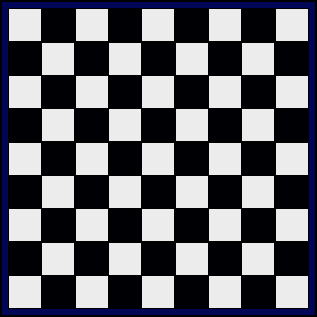
\includegraphics[width = 0.5\textwidth]{figures/img1}		
		\end{center}
		\only<+(1)>{\fillpic{height=\paperheight}{figures/img1}}
		%\pause % uncomment this, if you wanna jump back to the frame before zooming
	\end{frame}	
		
		
	\begin{frame}{Bildoverlap}{Absolutes Positionieren}
		Test \cite{art:whatsappnocosts}
		\pictureat{1cm}{2.5cm}{width = 6cm}{figures/img1}
		\pictureat{7.25cm}{2.5cm}{width = 4cm}{figures/img1}
		\pictureat{7.25cm}{5.75cm}{width = 4cm}{figures/img1}
	\end{frame}
	
	
	\begin{frame}{Bildoverlap}{Relatives Positionieren im Text}
		Hier könnte Ihre Werbung stehen! \cite{art:whatsappnocosts2}\dots und der Text geht tatsächlich weiter\\
		\begin{figure}
			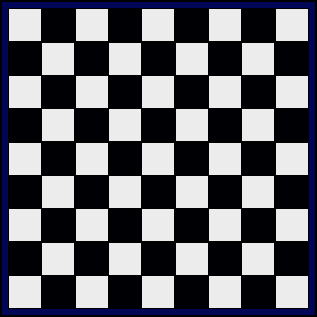
\includegraphics[height=3.35cm]{figures/img1}
			\raisebox{3cm}{\cite{art:swengineering1}}
		\end{figure}
		und auch nach dem Bild kommt noch sinnloses BlaBla
	\end{frame}
	
	
	\begin{frame}{Bildoverlap}
	\framesubtitle{Relatives Positionieren in einer Tabelle}
		\begin{center}%
		\begin{tabular}{cc}%
			\visible<+(1)->{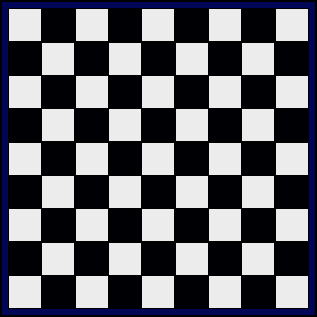
\includegraphics[width = 0.15\textwidth]{figures/img1}}&
			\visible<+(1)->{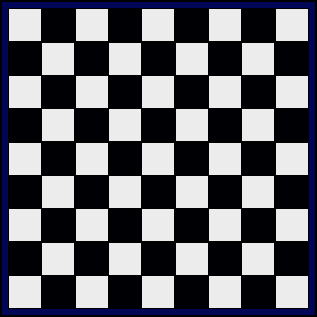
\includegraphics[width = 0.12\textwidth]{figures/img1}} \\
			\visible<+(1)->{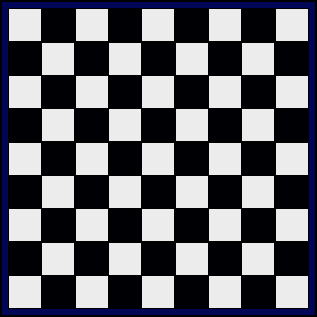
\includegraphics[width = 0.2\textwidth]{figures/img1}} &
			\visible<+(1)->{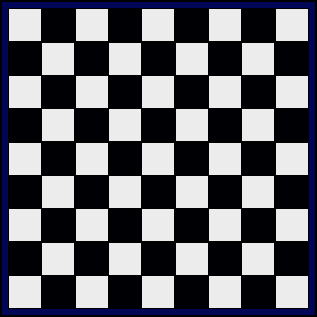
\includegraphics[width = 0.3\textwidth]{figures/img1}} \\
		\end{tabular}%
		\end{center}%
	\end{frame}
	
	
	% ##### don't forget to compile with biblatex #####
	\printbibliographyframe
	
\end{document}